\documentclass[letterpaper,12pt]{article}
\usepackage[margin=.65in,top=.72in,bottom=.62in,headheight=16pt,headsep=15pt,footskip=19pt]{geometry}
\usepackage[T1]{fontenc}
\usepackage{lmodern,tikz,fancyhdr}\pdfmapfile{+lm.map}
\usetikzlibrary{arrows.meta,shapes.geometric}
\pagestyle{fancy}\fancyhf{}\renewcommand{\headrulewidth}{0pt}\renewcommand{\footrulewidth}{0pt}
\setlength{\parindent}{0pt}\setlength{\parskip}{0pt}
\fancyhead[L]{\small Week 46 / Two boards forget their starts / Grades 4--5}
\fancyfoot[L]{\footnotesize Bellingham Math Circle / Week 46 / W46-grades-4-5-v2}\fancyfoot[R]{\footnotesize\thepage}
\begin{document}
\noindent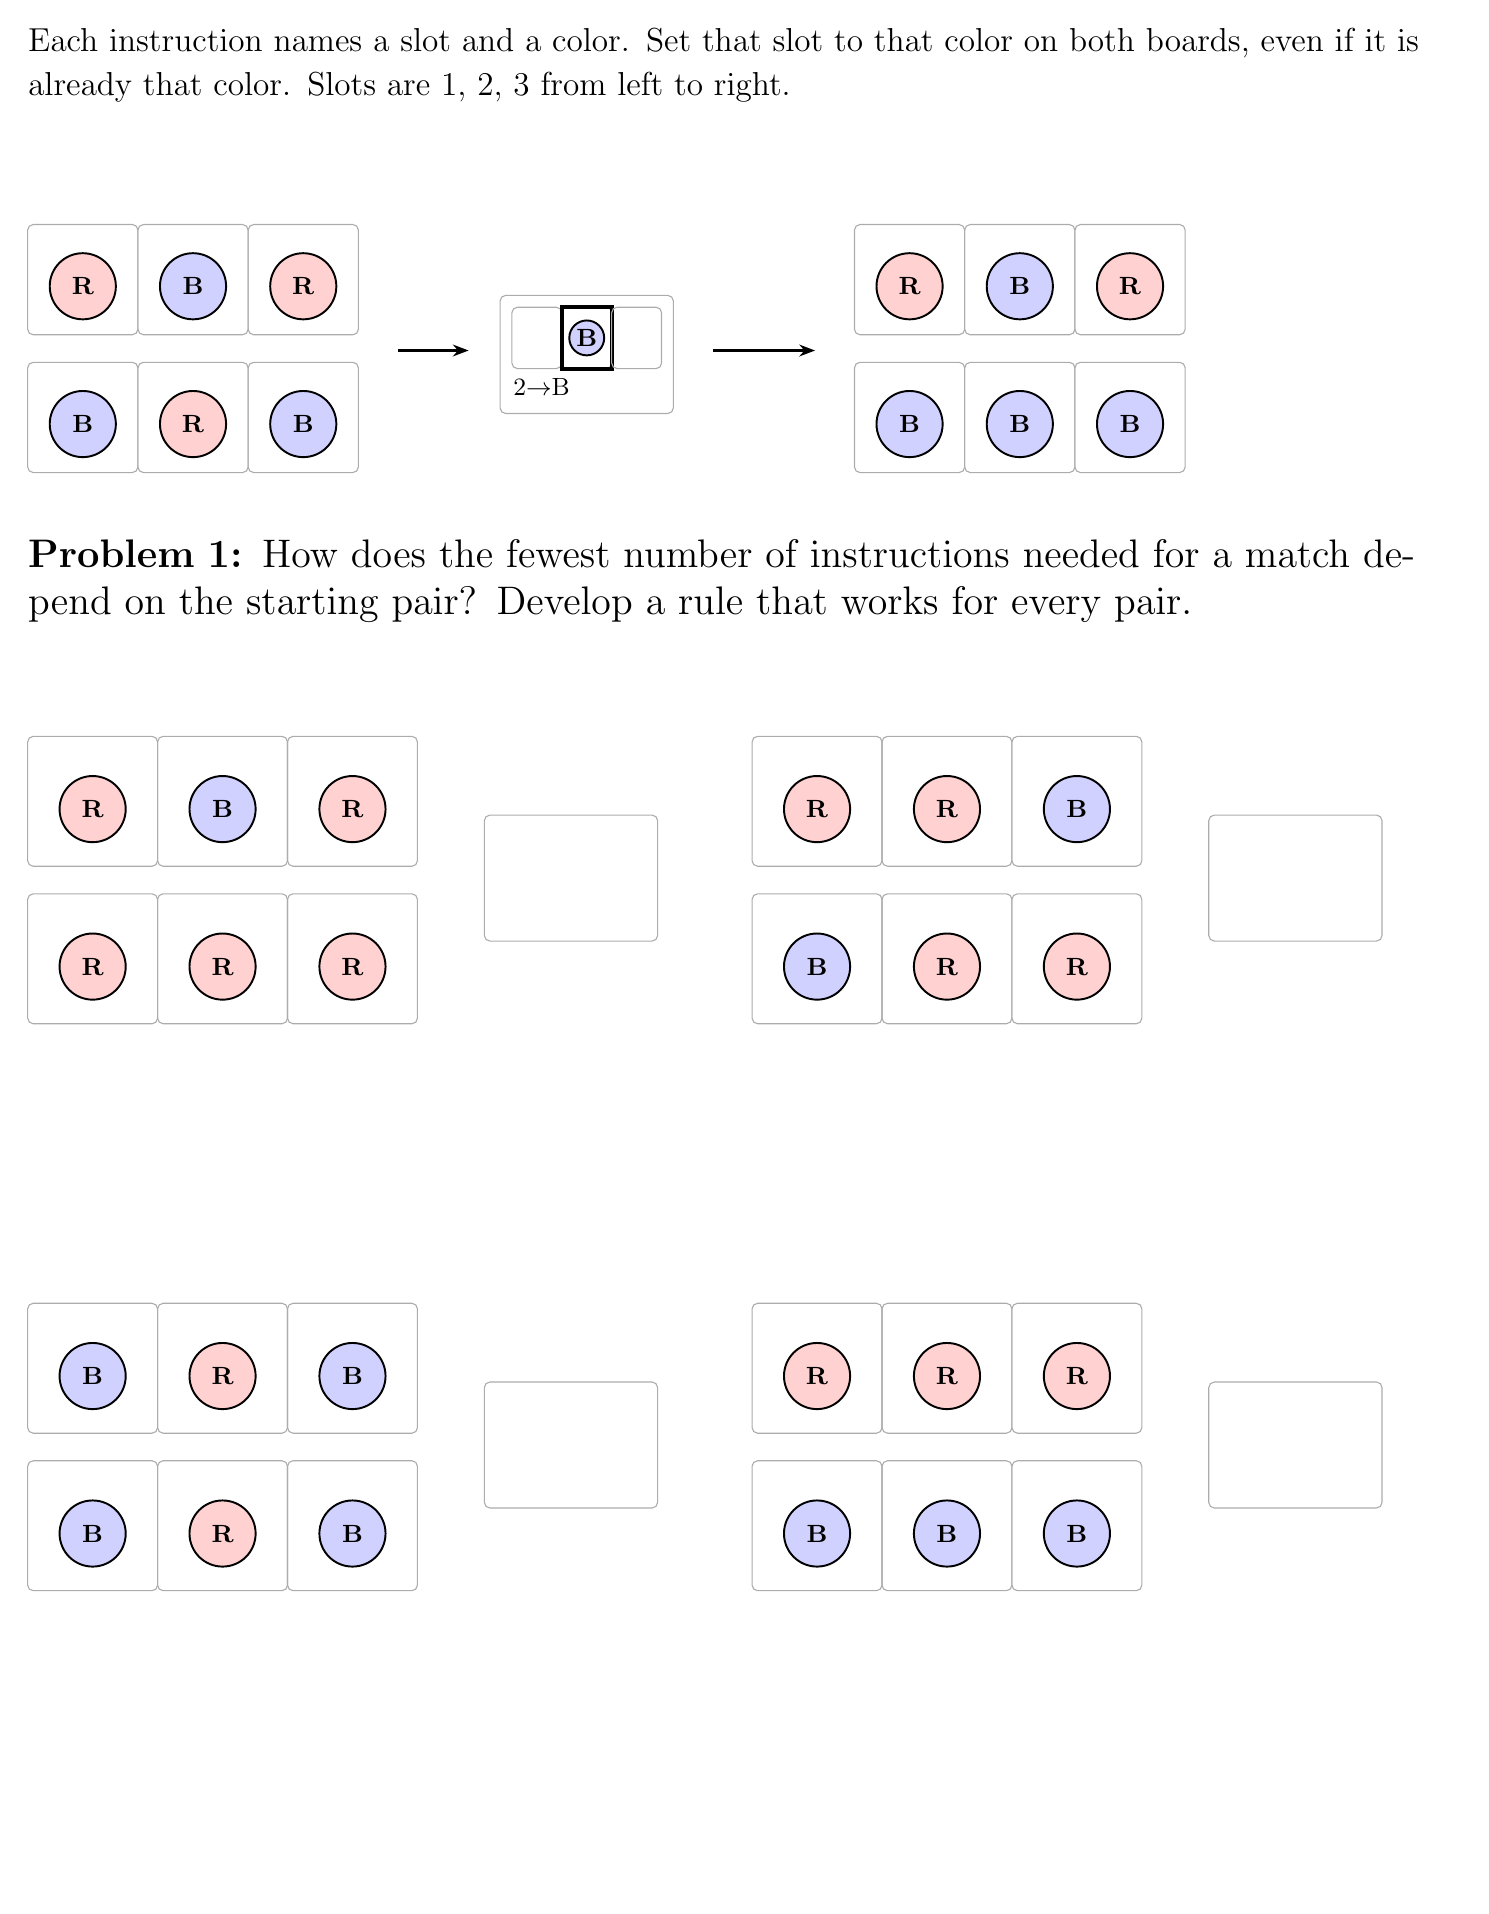
\begin{tikzpicture}[x=1cm,y=1cm]\path[use as bounding box] (0,0) rectangle (18.2,-23.6);
\node[anchor=north west,text width=18cm,inner sep=0pt,font=\fontsize{13}{16}\selectfont] at (0,0) {Each instruction names a slot and a color. Set that slot to that color on both boards, even if it is already that color. Slots are 1, 2, 3 from left to right.};
\draw[gray!65,rounded corners=2pt] (0.0,-2.5) rectangle (1.4,-3.9);
\draw[fill=red!18,line width=.7pt] (0.7,-3.284) circle (0.42);
\node[font=\bfseries\small] at (0.7,-3.284) {R};
\draw[gray!65,rounded corners=2pt] (1.4,-2.5) rectangle (2.8,-3.9);
\draw[fill=blue!18,line width=.7pt] (2.0999999999999996,-3.284) circle (0.42);
\node[font=\bfseries\small] at (2.0999999999999996,-3.284) {B};
\draw[gray!65,rounded corners=2pt] (2.8,-2.5) rectangle (4.199999999999999,-3.9);
\draw[fill=red!18,line width=.7pt] (3.5,-3.284) circle (0.42);
\node[font=\bfseries\small] at (3.5,-3.284) {R};
\draw[gray!65,rounded corners=2pt] (0.0,-4.25) rectangle (1.4,-5.65);
\draw[fill=blue!18,line width=.7pt] (0.7,-5.034) circle (0.42);
\node[font=\bfseries\small] at (0.7,-5.034) {B};
\draw[gray!65,rounded corners=2pt] (1.4,-4.25) rectangle (2.8,-5.65);
\draw[fill=red!18,line width=.7pt] (2.0999999999999996,-5.034) circle (0.42);
\node[font=\bfseries\small] at (2.0999999999999996,-5.034) {R};
\draw[gray!65,rounded corners=2pt] (2.8,-4.25) rectangle (4.199999999999999,-5.65);
\draw[fill=blue!18,line width=.7pt] (3.5,-5.034) circle (0.42);
\node[font=\bfseries\small] at (3.5,-5.034) {B};
\draw[gray!65,rounded corners=2pt] (6,-3.4) rectangle (8.2,-4.9);
\draw[gray!65,rounded corners=2pt] (6.15,-3.55) rectangle (6.783333333333334,-4.33);
\draw[gray!65,rounded corners=2pt] (6.783333333333334,-3.55) rectangle (7.416666666666668,-4.33);
\draw[line width=1.4pt] (6.783333333333334,-3.55) rectangle (7.416666666666668,-4.33);
\draw[fill=blue!18,line width=.7pt] (7.1000000000000005,-3.94) circle (0.22166666666666668);
\node[font=\bfseries\small] at (7.1000000000000005,-3.94) {B};
\draw[gray!65,rounded corners=2pt] (7.416666666666667,-3.55) rectangle (8.05,-4.33);
\node[anchor=north west,text width=2.0cm,inner sep=0pt,font=\fontsize{9}{12}\selectfont] at (6.16,-4.45) {2$\to$B};
\draw[-{Stealth[length=2mm]},line width=.8pt] (4.7,-4.1) -- (5.6,-4.1) node[midway,above,font=\small] {};
\draw[-{Stealth[length=2mm]},line width=.8pt] (8.7,-4.1) -- (10,-4.1) node[midway,above,font=\small] {};
\draw[gray!65,rounded corners=2pt] (10.5,-2.5) rectangle (11.9,-3.9);
\draw[fill=red!18,line width=.7pt] (11.2,-3.284) circle (0.42);
\node[font=\bfseries\small] at (11.2,-3.284) {R};
\draw[gray!65,rounded corners=2pt] (11.9,-2.5) rectangle (13.3,-3.9);
\draw[fill=blue!18,line width=.7pt] (12.6,-3.284) circle (0.42);
\node[font=\bfseries\small] at (12.6,-3.284) {B};
\draw[gray!65,rounded corners=2pt] (13.3,-2.5) rectangle (14.700000000000001,-3.9);
\draw[fill=red!18,line width=.7pt] (14.0,-3.284) circle (0.42);
\node[font=\bfseries\small] at (14.0,-3.284) {R};
\draw[gray!65,rounded corners=2pt] (10.5,-4.25) rectangle (11.9,-5.65);
\draw[fill=blue!18,line width=.7pt] (11.2,-5.034) circle (0.42);
\node[font=\bfseries\small] at (11.2,-5.034) {B};
\draw[gray!65,rounded corners=2pt] (11.9,-4.25) rectangle (13.3,-5.65);
\draw[fill=blue!18,line width=.7pt] (12.6,-5.034) circle (0.42);
\node[font=\bfseries\small] at (12.6,-5.034) {B};
\draw[gray!65,rounded corners=2pt] (13.3,-4.25) rectangle (14.700000000000001,-5.65);
\draw[fill=blue!18,line width=.7pt] (14.0,-5.034) circle (0.42);
\node[font=\bfseries\small] at (14.0,-5.034) {B};
\node[anchor=north west,text width=18cm,inner sep=0pt,font=\fontsize{14}{17}\selectfont] at (0,-6.5) {\textbf{Problem 1:} How does the fewest number of instructions needed for a match depend on the starting pair? Develop a rule that works for every pair.};
\draw[gray!65,rounded corners=2pt] (0.0,-9.0) rectangle (1.65,-10.65);
\draw[fill=red!18,line width=.7pt] (0.825,-9.924) circle (0.42);
\node[font=\bfseries\small] at (0.825,-9.924) {R};
\draw[gray!65,rounded corners=2pt] (1.65,-9.0) rectangle (3.3,-10.65);
\draw[fill=blue!18,line width=.7pt] (2.4749999999999996,-9.924) circle (0.42);
\node[font=\bfseries\small] at (2.4749999999999996,-9.924) {B};
\draw[gray!65,rounded corners=2pt] (3.3,-9.0) rectangle (4.949999999999999,-10.65);
\draw[fill=red!18,line width=.7pt] (4.125,-9.924) circle (0.42);
\node[font=\bfseries\small] at (4.125,-9.924) {R};
\draw[gray!65,rounded corners=2pt] (0.0,-11.0) rectangle (1.65,-12.65);
\draw[fill=red!18,line width=.7pt] (0.825,-11.924) circle (0.42);
\node[font=\bfseries\small] at (0.825,-11.924) {R};
\draw[gray!65,rounded corners=2pt] (1.65,-11.0) rectangle (3.3,-12.65);
\draw[fill=red!18,line width=.7pt] (2.4749999999999996,-11.924) circle (0.42);
\node[font=\bfseries\small] at (2.4749999999999996,-11.924) {R};
\draw[gray!65,rounded corners=2pt] (3.3,-11.0) rectangle (4.949999999999999,-12.65);
\draw[fill=red!18,line width=.7pt] (4.125,-11.924) circle (0.42);
\node[font=\bfseries\small] at (4.125,-11.924) {R};
\draw[gray!65,rounded corners=2pt] (5.8,-10.0) rectangle (8.0,-11.6);
\draw[gray!65,rounded corners=2pt] (9.2,-9.0) rectangle (10.85,-10.65);
\draw[fill=red!18,line width=.7pt] (10.024999999999999,-9.924) circle (0.42);
\node[font=\bfseries\small] at (10.024999999999999,-9.924) {R};
\draw[gray!65,rounded corners=2pt] (10.85,-9.0) rectangle (12.5,-10.65);
\draw[fill=red!18,line width=.7pt] (11.674999999999999,-9.924) circle (0.42);
\node[font=\bfseries\small] at (11.674999999999999,-9.924) {R};
\draw[gray!65,rounded corners=2pt] (12.5,-9.0) rectangle (14.15,-10.65);
\draw[fill=blue!18,line width=.7pt] (13.325,-9.924) circle (0.42);
\node[font=\bfseries\small] at (13.325,-9.924) {B};
\draw[gray!65,rounded corners=2pt] (9.2,-11.0) rectangle (10.85,-12.65);
\draw[fill=blue!18,line width=.7pt] (10.024999999999999,-11.924) circle (0.42);
\node[font=\bfseries\small] at (10.024999999999999,-11.924) {B};
\draw[gray!65,rounded corners=2pt] (10.85,-11.0) rectangle (12.5,-12.65);
\draw[fill=red!18,line width=.7pt] (11.674999999999999,-11.924) circle (0.42);
\node[font=\bfseries\small] at (11.674999999999999,-11.924) {R};
\draw[gray!65,rounded corners=2pt] (12.5,-11.0) rectangle (14.15,-12.65);
\draw[fill=red!18,line width=.7pt] (13.325,-11.924) circle (0.42);
\node[font=\bfseries\small] at (13.325,-11.924) {R};
\draw[gray!65,rounded corners=2pt] (15.0,-10.0) rectangle (17.2,-11.6);
\draw[gray!65,rounded corners=2pt] (0.0,-16.2) rectangle (1.65,-17.849999999999998);
\draw[fill=blue!18,line width=.7pt] (0.825,-17.124) circle (0.42);
\node[font=\bfseries\small] at (0.825,-17.124) {B};
\draw[gray!65,rounded corners=2pt] (1.65,-16.2) rectangle (3.3,-17.849999999999998);
\draw[fill=red!18,line width=.7pt] (2.4749999999999996,-17.124) circle (0.42);
\node[font=\bfseries\small] at (2.4749999999999996,-17.124) {R};
\draw[gray!65,rounded corners=2pt] (3.3,-16.2) rectangle (4.949999999999999,-17.849999999999998);
\draw[fill=blue!18,line width=.7pt] (4.125,-17.124) circle (0.42);
\node[font=\bfseries\small] at (4.125,-17.124) {B};
\draw[gray!65,rounded corners=2pt] (0.0,-18.2) rectangle (1.65,-19.849999999999998);
\draw[fill=blue!18,line width=.7pt] (0.825,-19.124) circle (0.42);
\node[font=\bfseries\small] at (0.825,-19.124) {B};
\draw[gray!65,rounded corners=2pt] (1.65,-18.2) rectangle (3.3,-19.849999999999998);
\draw[fill=red!18,line width=.7pt] (2.4749999999999996,-19.124) circle (0.42);
\node[font=\bfseries\small] at (2.4749999999999996,-19.124) {R};
\draw[gray!65,rounded corners=2pt] (3.3,-18.2) rectangle (4.949999999999999,-19.849999999999998);
\draw[fill=blue!18,line width=.7pt] (4.125,-19.124) circle (0.42);
\node[font=\bfseries\small] at (4.125,-19.124) {B};
\draw[gray!65,rounded corners=2pt] (5.8,-17.2) rectangle (8.0,-18.8);
\draw[gray!65,rounded corners=2pt] (9.2,-16.2) rectangle (10.85,-17.849999999999998);
\draw[fill=red!18,line width=.7pt] (10.024999999999999,-17.124) circle (0.42);
\node[font=\bfseries\small] at (10.024999999999999,-17.124) {R};
\draw[gray!65,rounded corners=2pt] (10.85,-16.2) rectangle (12.5,-17.849999999999998);
\draw[fill=red!18,line width=.7pt] (11.674999999999999,-17.124) circle (0.42);
\node[font=\bfseries\small] at (11.674999999999999,-17.124) {R};
\draw[gray!65,rounded corners=2pt] (12.5,-16.2) rectangle (14.15,-17.849999999999998);
\draw[fill=red!18,line width=.7pt] (13.325,-17.124) circle (0.42);
\node[font=\bfseries\small] at (13.325,-17.124) {R};
\draw[gray!65,rounded corners=2pt] (9.2,-18.2) rectangle (10.85,-19.849999999999998);
\draw[fill=blue!18,line width=.7pt] (10.024999999999999,-19.124) circle (0.42);
\node[font=\bfseries\small] at (10.024999999999999,-19.124) {B};
\draw[gray!65,rounded corners=2pt] (10.85,-18.2) rectangle (12.5,-19.849999999999998);
\draw[fill=blue!18,line width=.7pt] (11.674999999999999,-19.124) circle (0.42);
\node[font=\bfseries\small] at (11.674999999999999,-19.124) {B};
\draw[gray!65,rounded corners=2pt] (12.5,-18.2) rectangle (14.15,-19.849999999999998);
\draw[fill=blue!18,line width=.7pt] (13.325,-19.124) circle (0.42);
\node[font=\bfseries\small] at (13.325,-19.124) {B};
\draw[gray!65,rounded corners=2pt] (15.0,-17.2) rectangle (17.2,-18.8);
\end{tikzpicture}
\newpage
\noindent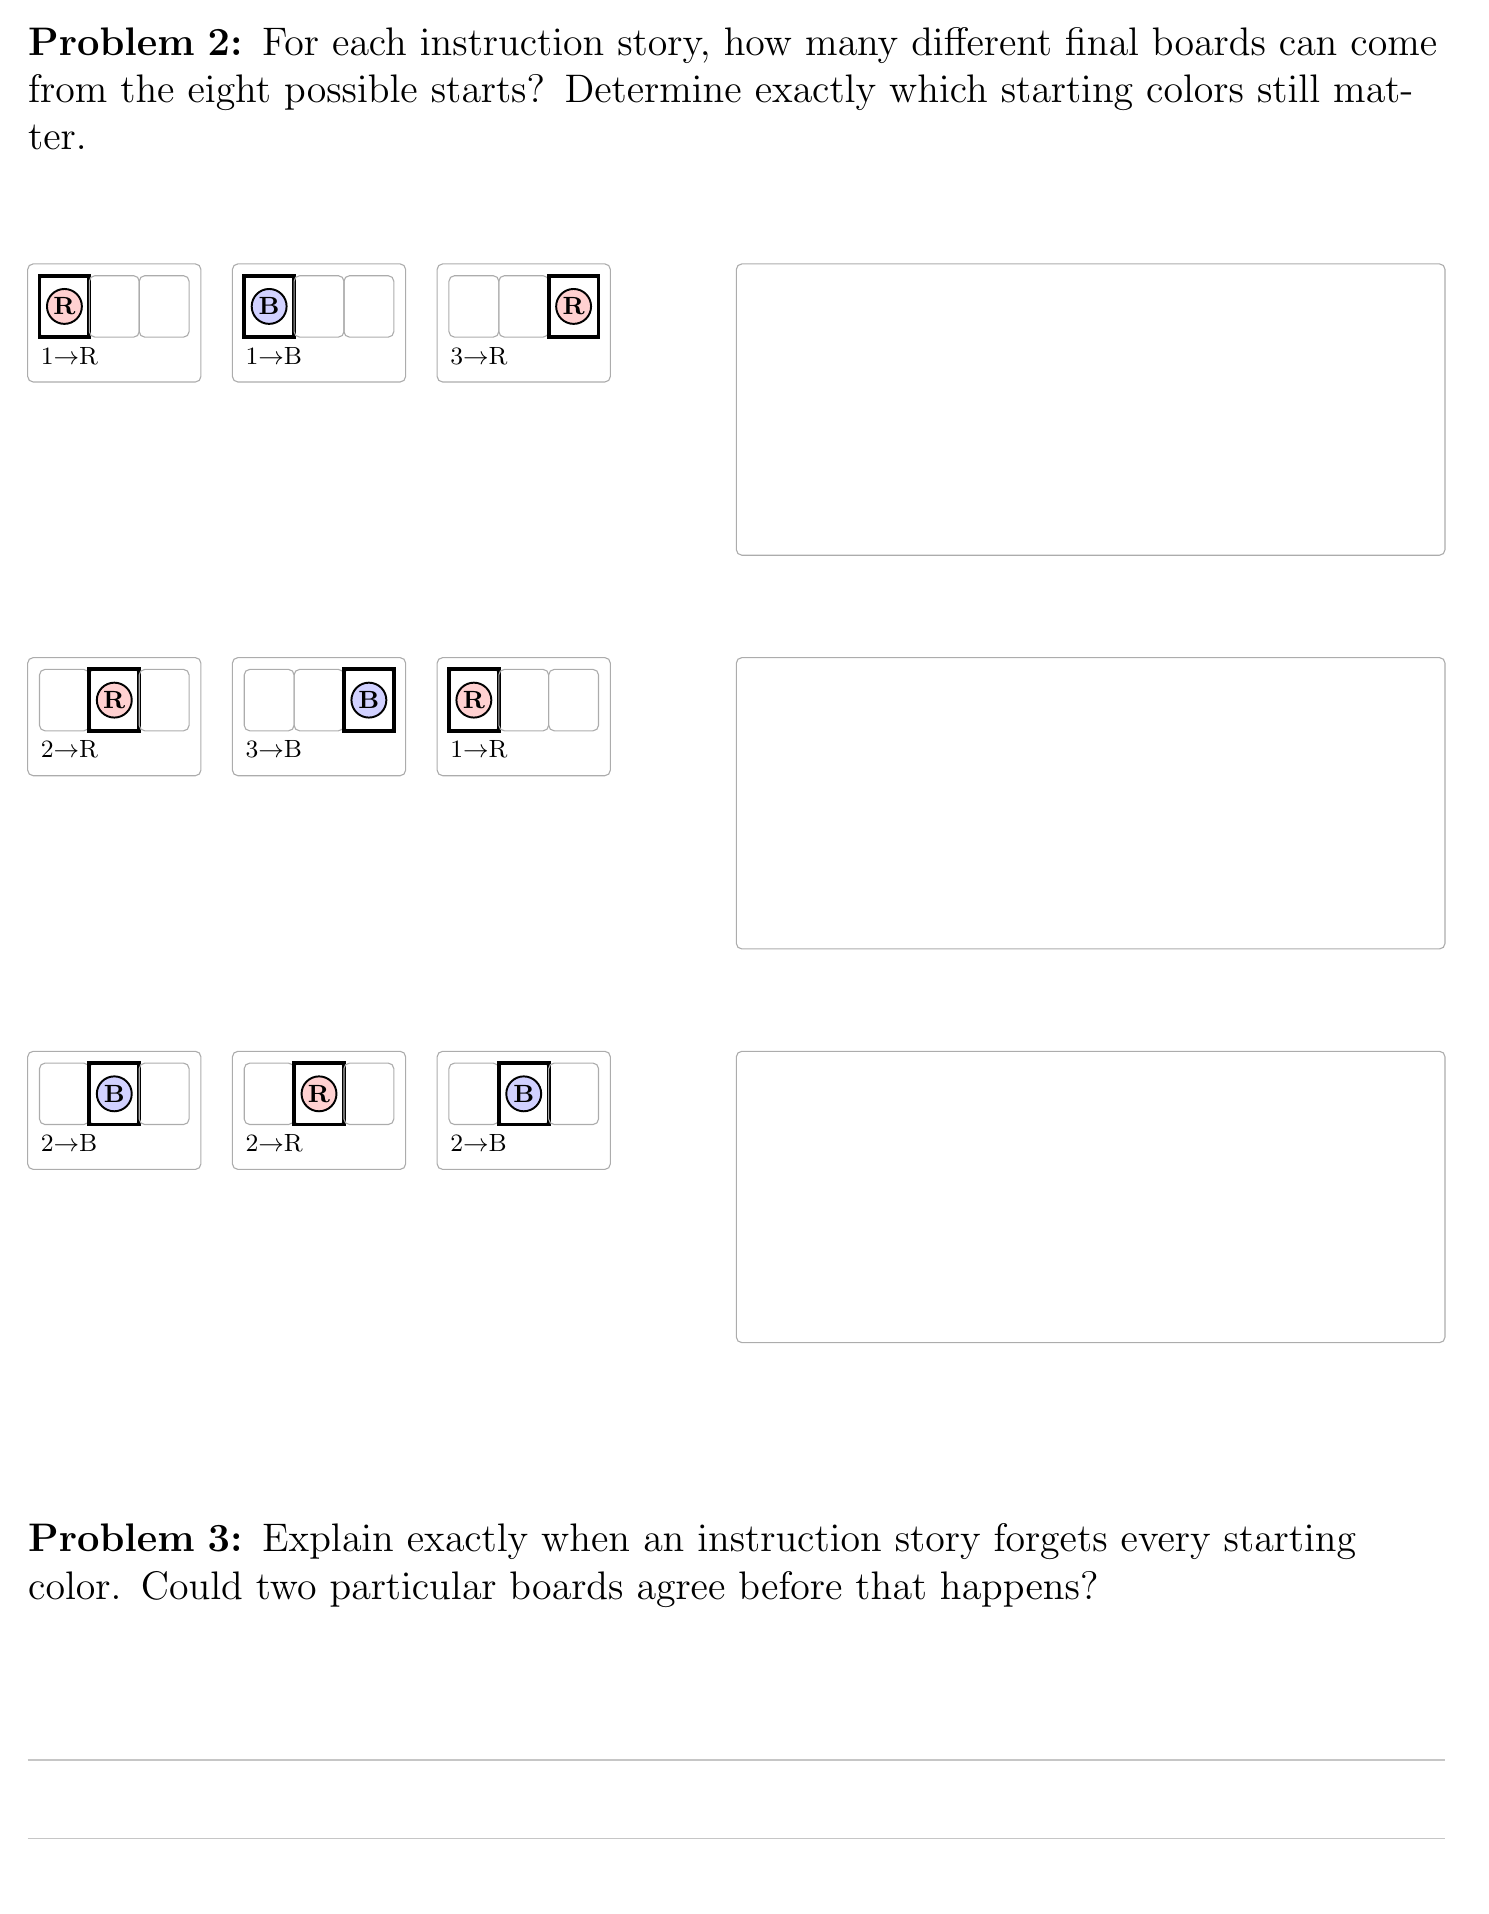
\begin{tikzpicture}[x=1cm,y=1cm]\path[use as bounding box] (0,0) rectangle (18.2,-23.6);
\node[anchor=north west,text width=18cm,inner sep=0pt,font=\fontsize{14}{17}\selectfont] at (0,0) {\textbf{Problem 2:} For each instruction story, how many different final boards can come from the eight possible starts? Determine exactly which starting colors still matter.};
\draw[gray!65,rounded corners=2pt] (0.0,-3) rectangle (2.2,-4.5);
\draw[gray!65,rounded corners=2pt] (0.15,-3.15) rectangle (0.7833333333333334,-3.9299999999999997);
\draw[line width=1.4pt] (0.15,-3.15) rectangle (0.7833333333333334,-3.93);
\draw[fill=red!18,line width=.7pt] (0.4666666666666667,-3.54) circle (0.22166666666666668);
\node[font=\bfseries\small] at (0.4666666666666667,-3.54) {R};
\draw[gray!65,rounded corners=2pt] (0.7833333333333334,-3.15) rectangle (1.416666666666667,-3.9299999999999997);
\draw[gray!65,rounded corners=2pt] (1.4166666666666667,-3.15) rectangle (2.0500000000000003,-3.9299999999999997);
\node[anchor=north west,text width=2.0cm,inner sep=0pt,font=\fontsize{9}{12}\selectfont] at (0.16,-4.05) {1$\to$R};
\draw[gray!65,rounded corners=2pt] (2.6,-3) rectangle (4.800000000000001,-4.5);
\draw[gray!65,rounded corners=2pt] (2.75,-3.15) rectangle (3.3833333333333333,-3.9299999999999997);
\draw[line width=1.4pt] (2.75,-3.15) rectangle (3.3833333333333333,-3.93);
\draw[fill=blue!18,line width=.7pt] (3.066666666666667,-3.54) circle (0.22166666666666668);
\node[font=\bfseries\small] at (3.066666666666667,-3.54) {B};
\draw[gray!65,rounded corners=2pt] (3.3833333333333333,-3.15) rectangle (4.016666666666667,-3.9299999999999997);
\draw[gray!65,rounded corners=2pt] (4.016666666666667,-3.15) rectangle (4.65,-3.9299999999999997);
\node[anchor=north west,text width=2.0cm,inner sep=0pt,font=\fontsize{9}{12}\selectfont] at (2.7600000000000002,-4.05) {1$\to$B};
\draw[gray!65,rounded corners=2pt] (5.2,-3) rectangle (7.4,-4.5);
\draw[gray!65,rounded corners=2pt] (5.3500000000000005,-3.15) rectangle (5.983333333333334,-3.9299999999999997);
\draw[gray!65,rounded corners=2pt] (5.983333333333334,-3.15) rectangle (6.616666666666668,-3.9299999999999997);
\draw[gray!65,rounded corners=2pt] (6.616666666666667,-3.15) rectangle (7.250000000000001,-3.9299999999999997);
\draw[line width=1.4pt] (6.616666666666667,-3.15) rectangle (7.250000000000001,-3.93);
\draw[fill=red!18,line width=.7pt] (6.933333333333334,-3.54) circle (0.22166666666666668);
\node[font=\bfseries\small] at (6.933333333333334,-3.54) {R};
\node[anchor=north west,text width=2.0cm,inner sep=0pt,font=\fontsize{9}{12}\selectfont] at (5.36,-4.05) {3$\to$R};
\draw[gray!65,rounded corners=2pt] (9,-3) rectangle (18,-6.7);
\draw[gray!65,rounded corners=2pt] (0.0,-8) rectangle (2.2,-9.5);
\draw[gray!65,rounded corners=2pt] (0.15,-8.15) rectangle (0.7833333333333334,-8.93);
\draw[gray!65,rounded corners=2pt] (0.7833333333333334,-8.15) rectangle (1.416666666666667,-8.93);
\draw[line width=1.4pt] (0.7833333333333334,-8.15) rectangle (1.416666666666667,-8.93);
\draw[fill=red!18,line width=.7pt] (1.1,-8.54) circle (0.22166666666666668);
\node[font=\bfseries\small] at (1.1,-8.54) {R};
\draw[gray!65,rounded corners=2pt] (1.4166666666666667,-8.15) rectangle (2.0500000000000003,-8.93);
\node[anchor=north west,text width=2.0cm,inner sep=0pt,font=\fontsize{9}{12}\selectfont] at (0.16,-9.05) {2$\to$R};
\draw[gray!65,rounded corners=2pt] (2.6,-8) rectangle (4.800000000000001,-9.5);
\draw[gray!65,rounded corners=2pt] (2.75,-8.15) rectangle (3.3833333333333333,-8.93);
\draw[gray!65,rounded corners=2pt] (3.3833333333333333,-8.15) rectangle (4.016666666666667,-8.93);
\draw[gray!65,rounded corners=2pt] (4.016666666666667,-8.15) rectangle (4.65,-8.93);
\draw[line width=1.4pt] (4.016666666666667,-8.15) rectangle (4.65,-8.93);
\draw[fill=blue!18,line width=.7pt] (4.333333333333333,-8.54) circle (0.22166666666666668);
\node[font=\bfseries\small] at (4.333333333333333,-8.54) {B};
\node[anchor=north west,text width=2.0cm,inner sep=0pt,font=\fontsize{9}{12}\selectfont] at (2.7600000000000002,-9.05) {3$\to$B};
\draw[gray!65,rounded corners=2pt] (5.2,-8) rectangle (7.4,-9.5);
\draw[gray!65,rounded corners=2pt] (5.3500000000000005,-8.15) rectangle (5.983333333333334,-8.93);
\draw[line width=1.4pt] (5.3500000000000005,-8.15) rectangle (5.983333333333334,-8.93);
\draw[fill=red!18,line width=.7pt] (5.666666666666667,-8.54) circle (0.22166666666666668);
\node[font=\bfseries\small] at (5.666666666666667,-8.54) {R};
\draw[gray!65,rounded corners=2pt] (5.983333333333334,-8.15) rectangle (6.616666666666668,-8.93);
\draw[gray!65,rounded corners=2pt] (6.616666666666667,-8.15) rectangle (7.250000000000001,-8.93);
\node[anchor=north west,text width=2.0cm,inner sep=0pt,font=\fontsize{9}{12}\selectfont] at (5.36,-9.05) {1$\to$R};
\draw[gray!65,rounded corners=2pt] (9,-8) rectangle (18,-11.7);
\draw[gray!65,rounded corners=2pt] (0.0,-13) rectangle (2.2,-14.5);
\draw[gray!65,rounded corners=2pt] (0.15,-13.15) rectangle (0.7833333333333334,-13.93);
\draw[gray!65,rounded corners=2pt] (0.7833333333333334,-13.15) rectangle (1.416666666666667,-13.93);
\draw[line width=1.4pt] (0.7833333333333334,-13.15) rectangle (1.416666666666667,-13.93);
\draw[fill=blue!18,line width=.7pt] (1.1,-13.54) circle (0.22166666666666668);
\node[font=\bfseries\small] at (1.1,-13.54) {B};
\draw[gray!65,rounded corners=2pt] (1.4166666666666667,-13.15) rectangle (2.0500000000000003,-13.93);
\node[anchor=north west,text width=2.0cm,inner sep=0pt,font=\fontsize{9}{12}\selectfont] at (0.16,-14.05) {2$\to$B};
\draw[gray!65,rounded corners=2pt] (2.6,-13) rectangle (4.800000000000001,-14.5);
\draw[gray!65,rounded corners=2pt] (2.75,-13.15) rectangle (3.3833333333333333,-13.93);
\draw[gray!65,rounded corners=2pt] (3.3833333333333333,-13.15) rectangle (4.016666666666667,-13.93);
\draw[line width=1.4pt] (3.3833333333333333,-13.15) rectangle (4.016666666666667,-13.93);
\draw[fill=red!18,line width=.7pt] (3.7,-13.54) circle (0.22166666666666668);
\node[font=\bfseries\small] at (3.7,-13.54) {R};
\draw[gray!65,rounded corners=2pt] (4.016666666666667,-13.15) rectangle (4.65,-13.93);
\node[anchor=north west,text width=2.0cm,inner sep=0pt,font=\fontsize{9}{12}\selectfont] at (2.7600000000000002,-14.05) {2$\to$R};
\draw[gray!65,rounded corners=2pt] (5.2,-13) rectangle (7.4,-14.5);
\draw[gray!65,rounded corners=2pt] (5.3500000000000005,-13.15) rectangle (5.983333333333334,-13.93);
\draw[gray!65,rounded corners=2pt] (5.983333333333334,-13.15) rectangle (6.616666666666668,-13.93);
\draw[line width=1.4pt] (5.983333333333334,-13.15) rectangle (6.616666666666668,-13.93);
\draw[fill=blue!18,line width=.7pt] (6.300000000000001,-13.54) circle (0.22166666666666668);
\node[font=\bfseries\small] at (6.300000000000001,-13.54) {B};
\draw[gray!65,rounded corners=2pt] (6.616666666666667,-13.15) rectangle (7.250000000000001,-13.93);
\node[anchor=north west,text width=2.0cm,inner sep=0pt,font=\fontsize{9}{12}\selectfont] at (5.36,-14.05) {2$\to$B};
\draw[gray!65,rounded corners=2pt] (9,-13) rectangle (18,-16.7);
\node[anchor=north west,text width=18cm,inner sep=0pt,font=\fontsize{14}{17}\selectfont] at (0,-19) {\textbf{Problem 3:} Explain exactly when an instruction story forgets every starting color. Could two particular boards agree before that happens?};
\draw[gray!45] (0,-22) -- (18,-22);
\draw[gray!45] (0,-23) -- (18,-23);
\end{tikzpicture}
\newpage
\noindent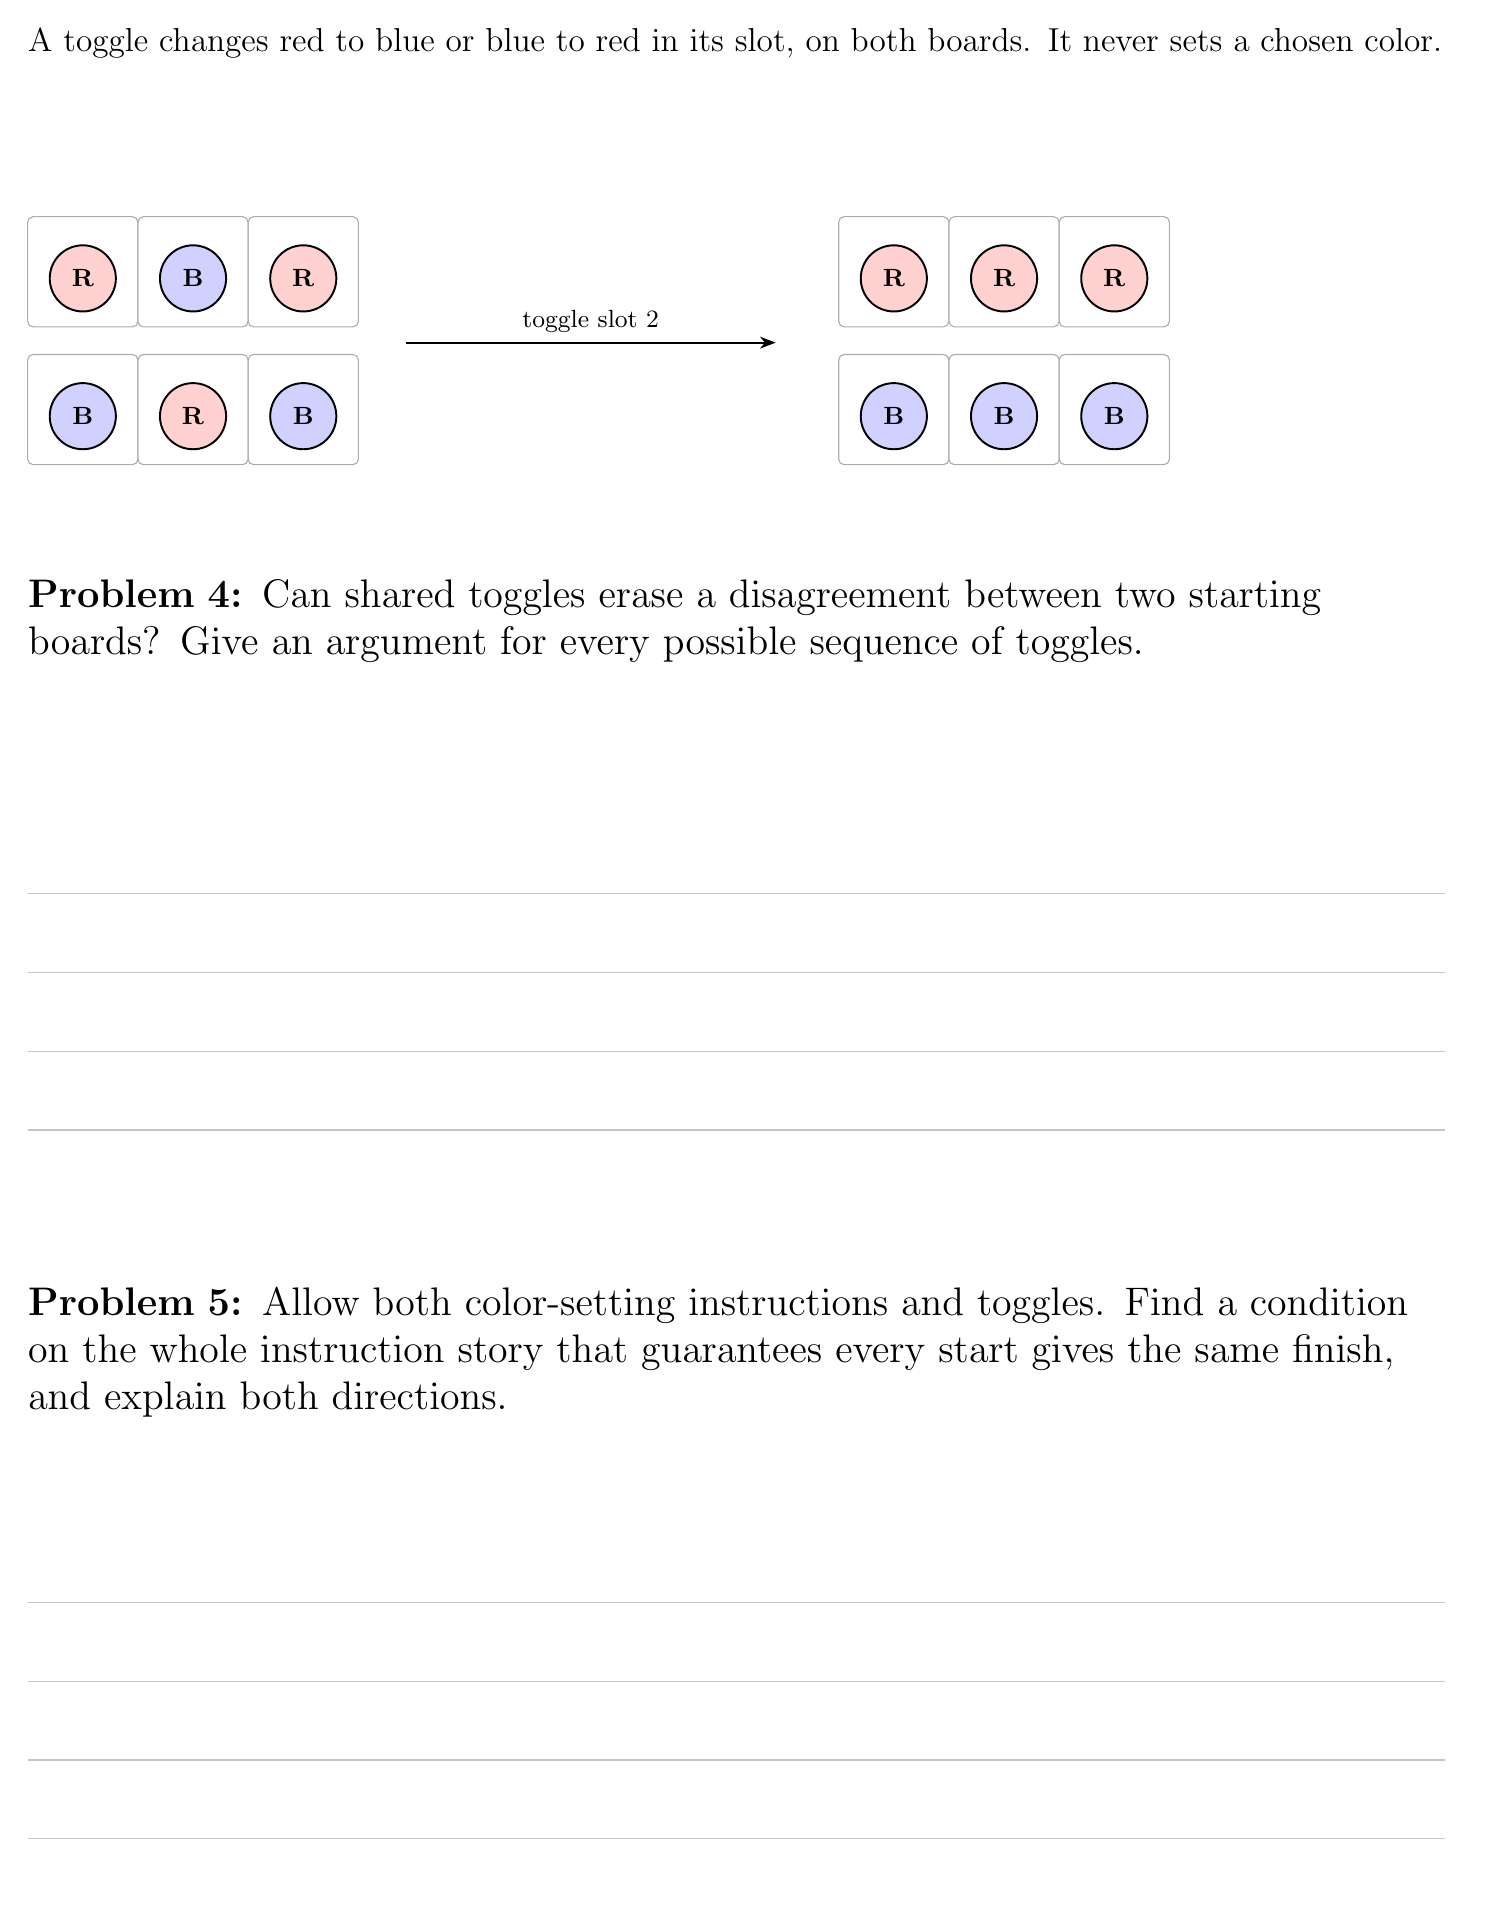
\begin{tikzpicture}[x=1cm,y=1cm]\path[use as bounding box] (0,0) rectangle (18.2,-23.6);
\node[anchor=north west,text width=18cm,inner sep=0pt,font=\fontsize{13}{16}\selectfont] at (0,0) {A toggle changes red to blue or blue to red in its slot, on both boards. It never sets a chosen color.};
\draw[gray!65,rounded corners=2pt] (0.0,-2.4) rectangle (1.4,-3.8);
\draw[fill=red!18,line width=.7pt] (0.7,-3.184) circle (0.42);
\node[font=\bfseries\small] at (0.7,-3.184) {R};
\draw[gray!65,rounded corners=2pt] (1.4,-2.4) rectangle (2.8,-3.8);
\draw[fill=blue!18,line width=.7pt] (2.0999999999999996,-3.184) circle (0.42);
\node[font=\bfseries\small] at (2.0999999999999996,-3.184) {B};
\draw[gray!65,rounded corners=2pt] (2.8,-2.4) rectangle (4.199999999999999,-3.8);
\draw[fill=red!18,line width=.7pt] (3.5,-3.184) circle (0.42);
\node[font=\bfseries\small] at (3.5,-3.184) {R};
\draw[gray!65,rounded corners=2pt] (0.0,-4.1499999999999995) rectangle (1.4,-5.549999999999999);
\draw[fill=blue!18,line width=.7pt] (0.7,-4.933999999999999) circle (0.42);
\node[font=\bfseries\small] at (0.7,-4.933999999999999) {B};
\draw[gray!65,rounded corners=2pt] (1.4,-4.1499999999999995) rectangle (2.8,-5.549999999999999);
\draw[fill=red!18,line width=.7pt] (2.0999999999999996,-4.933999999999999) circle (0.42);
\node[font=\bfseries\small] at (2.0999999999999996,-4.933999999999999) {R};
\draw[gray!65,rounded corners=2pt] (2.8,-4.1499999999999995) rectangle (4.199999999999999,-5.549999999999999);
\draw[fill=blue!18,line width=.7pt] (3.5,-4.933999999999999) circle (0.42);
\node[font=\bfseries\small] at (3.5,-4.933999999999999) {B};
\draw[-{Stealth[length=2mm]},line width=.8pt] (4.8,-4) -- (9.5,-4) node[midway,above,font=\small] {toggle slot 2};
\draw[gray!65,rounded corners=2pt] (10.3,-2.4) rectangle (11.700000000000001,-3.8);
\draw[fill=red!18,line width=.7pt] (11.0,-3.184) circle (0.42);
\node[font=\bfseries\small] at (11.0,-3.184) {R};
\draw[gray!65,rounded corners=2pt] (11.700000000000001,-2.4) rectangle (13.100000000000001,-3.8);
\draw[fill=red!18,line width=.7pt] (12.4,-3.184) circle (0.42);
\node[font=\bfseries\small] at (12.4,-3.184) {R};
\draw[gray!65,rounded corners=2pt] (13.100000000000001,-2.4) rectangle (14.500000000000002,-3.8);
\draw[fill=red!18,line width=.7pt] (13.8,-3.184) circle (0.42);
\node[font=\bfseries\small] at (13.8,-3.184) {R};
\draw[gray!65,rounded corners=2pt] (10.3,-4.1499999999999995) rectangle (11.700000000000001,-5.549999999999999);
\draw[fill=blue!18,line width=.7pt] (11.0,-4.933999999999999) circle (0.42);
\node[font=\bfseries\small] at (11.0,-4.933999999999999) {B};
\draw[gray!65,rounded corners=2pt] (11.700000000000001,-4.1499999999999995) rectangle (13.100000000000001,-5.549999999999999);
\draw[fill=blue!18,line width=.7pt] (12.4,-4.933999999999999) circle (0.42);
\node[font=\bfseries\small] at (12.4,-4.933999999999999) {B};
\draw[gray!65,rounded corners=2pt] (13.100000000000001,-4.1499999999999995) rectangle (14.500000000000002,-5.549999999999999);
\draw[fill=blue!18,line width=.7pt] (13.8,-4.933999999999999) circle (0.42);
\node[font=\bfseries\small] at (13.8,-4.933999999999999) {B};
\node[anchor=north west,text width=18cm,inner sep=0pt,font=\fontsize{14}{17}\selectfont] at (0,-7) {\textbf{Problem 4:} Can shared toggles erase a disagreement between two starting boards? Give an argument for every possible sequence of toggles.};
\draw[gray!45] (0,-11) -- (18,-11);
\draw[gray!45] (0,-12) -- (18,-12);
\draw[gray!45] (0,-13) -- (18,-13);
\draw[gray!45] (0,-14) -- (18,-14);
\node[anchor=north west,text width=18cm,inner sep=0pt,font=\fontsize{14}{17}\selectfont] at (0,-16) {\textbf{Problem 5:} Allow both color-setting instructions and toggles. Find a condition on the whole instruction story that guarantees every start gives the same finish, and explain both directions.};
\draw[gray!45] (0,-20) -- (18,-20);
\draw[gray!45] (0,-21) -- (18,-21);
\draw[gray!45] (0,-22) -- (18,-22);
\draw[gray!45] (0,-23) -- (18,-23);
\end{tikzpicture}
\newpage
\noindent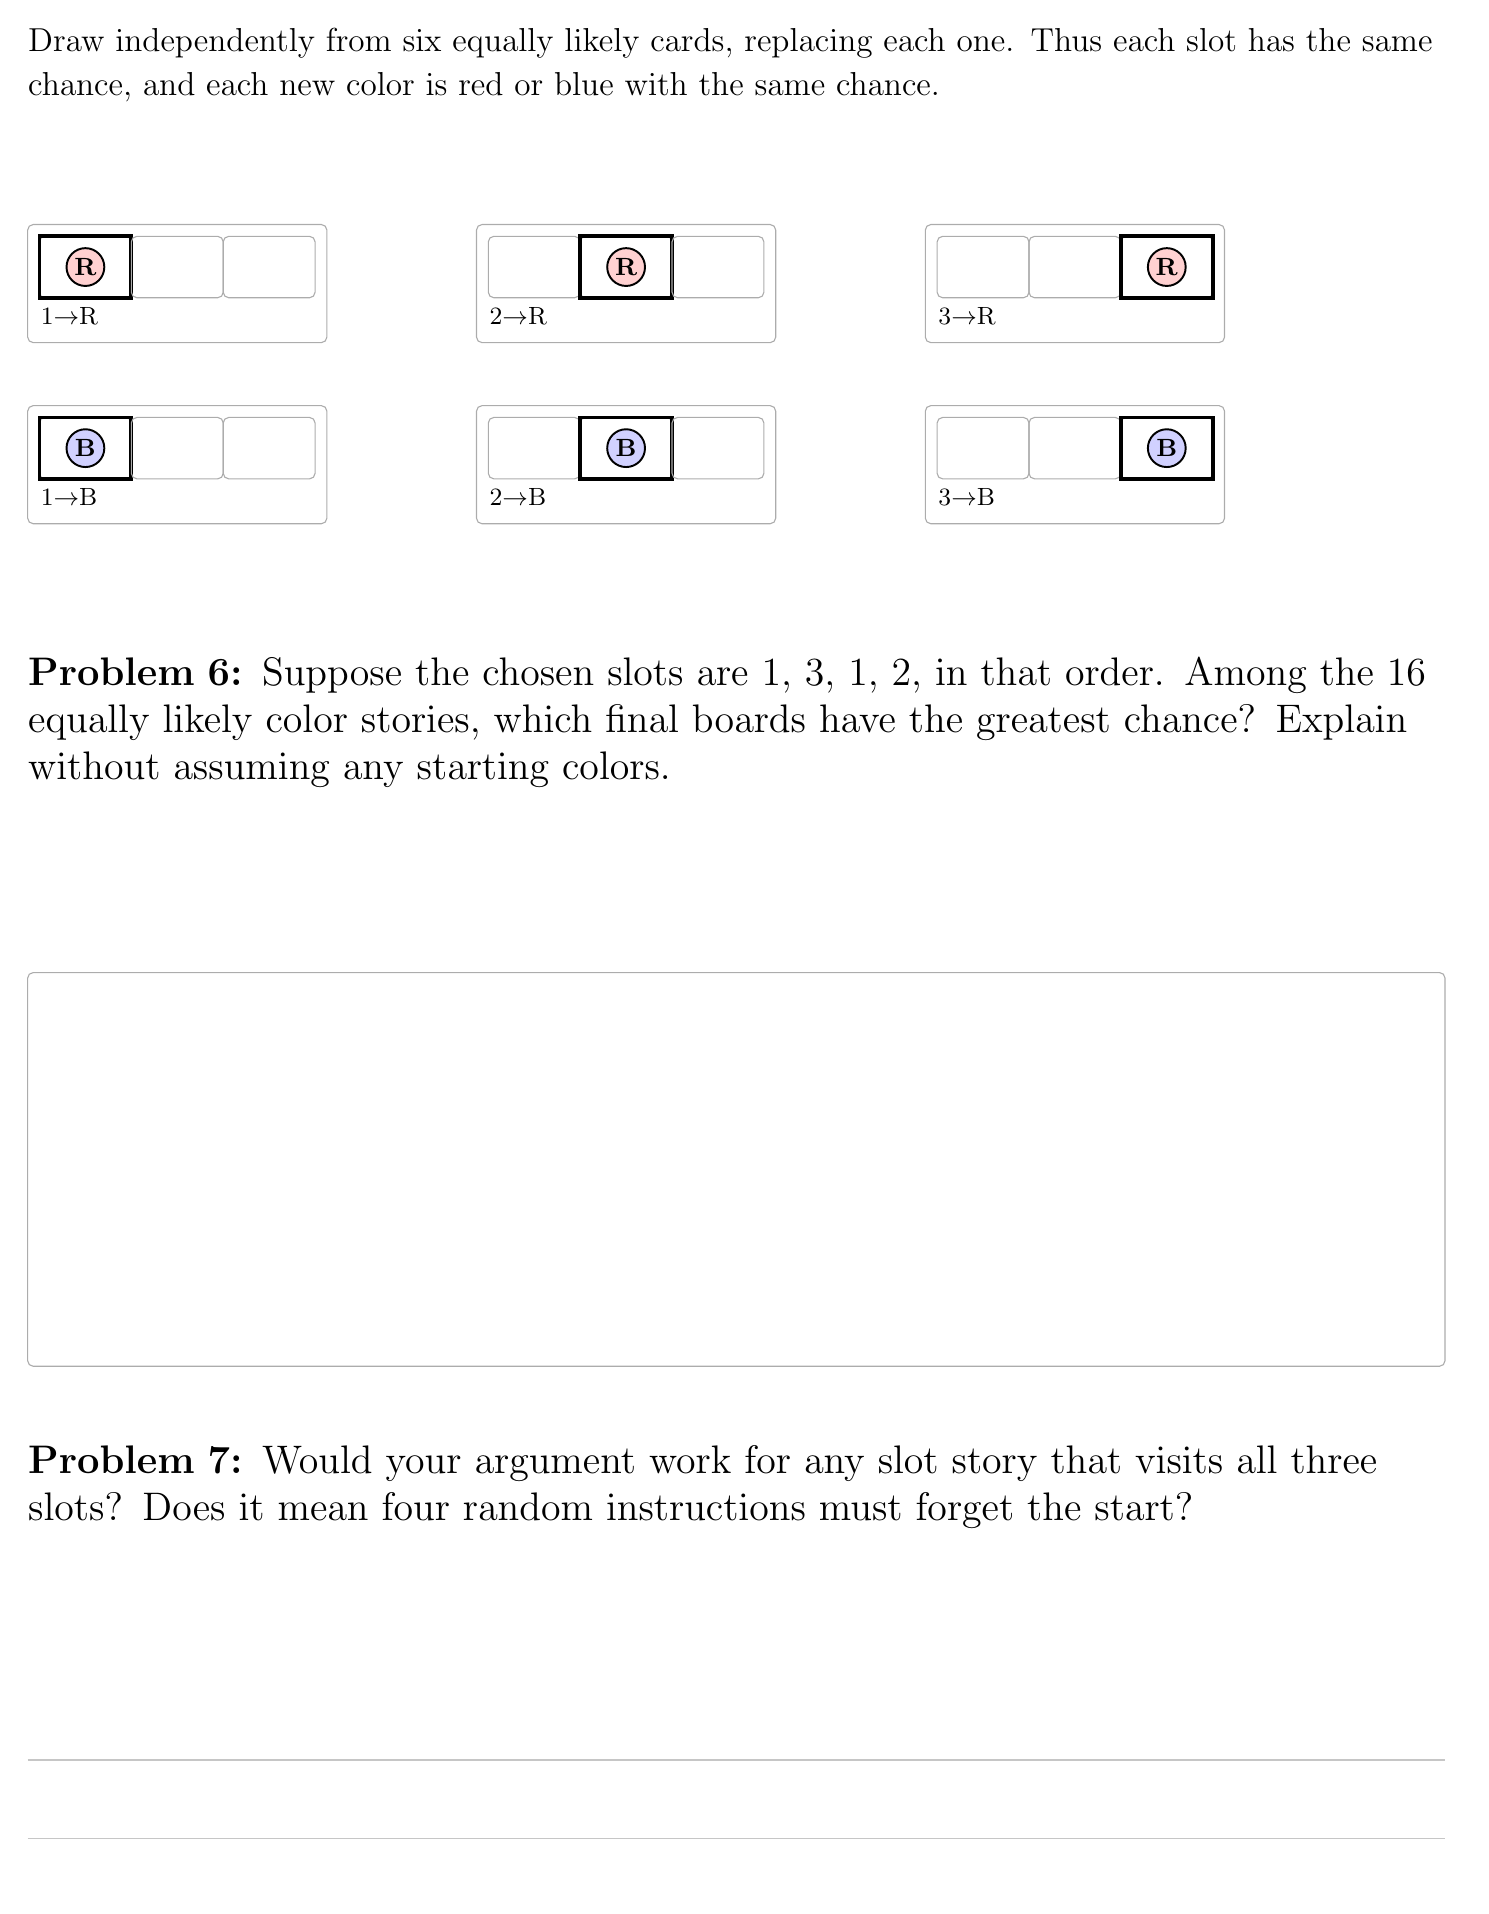
\begin{tikzpicture}[x=1cm,y=1cm]\path[use as bounding box] (0,0) rectangle (18.2,-23.6);
\node[anchor=north west,text width=18cm,inner sep=0pt,font=\fontsize{13}{16}\selectfont] at (0,0) {Draw independently from six equally likely cards, replacing each one. Thus each slot has the same chance, and each new color is red or blue with the same chance.};
\draw[gray!65,rounded corners=2pt] (0.0,-2.5) rectangle (3.8,-4.0);
\draw[gray!65,rounded corners=2pt] (0.15,-2.65) rectangle (1.3166666666666667,-3.4299999999999997);
\draw[line width=1.4pt] (0.15,-2.65) rectangle (1.3166666666666667,-3.43);
\draw[fill=red!18,line width=.7pt] (0.7333333333333334,-3.04) circle (0.24);
\node[font=\bfseries\small] at (0.7333333333333334,-3.04) {R};
\draw[gray!65,rounded corners=2pt] (1.3166666666666667,-2.65) rectangle (2.4833333333333334,-3.4299999999999997);
\draw[gray!65,rounded corners=2pt] (2.4833333333333334,-2.65) rectangle (3.6500000000000004,-3.4299999999999997);
\node[anchor=north west,text width=3.5999999999999996cm,inner sep=0pt,font=\fontsize{9}{12}\selectfont] at (0.16,-3.55) {1$\to$R};
\draw[gray!65,rounded corners=2pt] (5.7,-2.5) rectangle (9.5,-4.0);
\draw[gray!65,rounded corners=2pt] (5.8500000000000005,-2.65) rectangle (7.0166666666666675,-3.4299999999999997);
\draw[gray!65,rounded corners=2pt] (7.0166666666666675,-2.65) rectangle (8.183333333333334,-3.4299999999999997);
\draw[line width=1.4pt] (7.0166666666666675,-2.65) rectangle (8.183333333333334,-3.43);
\draw[fill=red!18,line width=.7pt] (7.6000000000000005,-3.04) circle (0.24);
\node[font=\bfseries\small] at (7.6000000000000005,-3.04) {R};
\draw[gray!65,rounded corners=2pt] (8.183333333333334,-2.65) rectangle (9.35,-3.4299999999999997);
\node[anchor=north west,text width=3.5999999999999996cm,inner sep=0pt,font=\fontsize{9}{12}\selectfont] at (5.86,-3.55) {2$\to$R};
\draw[gray!65,rounded corners=2pt] (11.4,-2.5) rectangle (15.2,-4.0);
\draw[gray!65,rounded corners=2pt] (11.55,-2.65) rectangle (12.716666666666667,-3.4299999999999997);
\draw[gray!65,rounded corners=2pt] (12.716666666666667,-2.65) rectangle (13.883333333333333,-3.4299999999999997);
\draw[gray!65,rounded corners=2pt] (13.883333333333335,-2.65) rectangle (15.05,-3.4299999999999997);
\draw[line width=1.4pt] (13.883333333333335,-2.65) rectangle (15.05,-3.43);
\draw[fill=red!18,line width=.7pt] (14.466666666666669,-3.04) circle (0.24);
\node[font=\bfseries\small] at (14.466666666666669,-3.04) {R};
\node[anchor=north west,text width=3.5999999999999996cm,inner sep=0pt,font=\fontsize{9}{12}\selectfont] at (11.56,-3.55) {3$\to$R};
\draw[gray!65,rounded corners=2pt] (0.0,-4.8) rectangle (3.8,-6.3);
\draw[gray!65,rounded corners=2pt] (0.15,-4.95) rectangle (1.3166666666666667,-5.73);
\draw[line width=1.4pt] (0.15,-4.95) rectangle (1.3166666666666667,-5.7299999999999995);
\draw[fill=blue!18,line width=.7pt] (0.7333333333333334,-5.34) circle (0.24);
\node[font=\bfseries\small] at (0.7333333333333334,-5.34) {B};
\draw[gray!65,rounded corners=2pt] (1.3166666666666667,-4.95) rectangle (2.4833333333333334,-5.73);
\draw[gray!65,rounded corners=2pt] (2.4833333333333334,-4.95) rectangle (3.6500000000000004,-5.73);
\node[anchor=north west,text width=3.5999999999999996cm,inner sep=0pt,font=\fontsize{9}{12}\selectfont] at (0.16,-5.85) {1$\to$B};
\draw[gray!65,rounded corners=2pt] (5.7,-4.8) rectangle (9.5,-6.3);
\draw[gray!65,rounded corners=2pt] (5.8500000000000005,-4.95) rectangle (7.0166666666666675,-5.73);
\draw[gray!65,rounded corners=2pt] (7.0166666666666675,-4.95) rectangle (8.183333333333334,-5.73);
\draw[line width=1.4pt] (7.0166666666666675,-4.95) rectangle (8.183333333333334,-5.7299999999999995);
\draw[fill=blue!18,line width=.7pt] (7.6000000000000005,-5.34) circle (0.24);
\node[font=\bfseries\small] at (7.6000000000000005,-5.34) {B};
\draw[gray!65,rounded corners=2pt] (8.183333333333334,-4.95) rectangle (9.35,-5.73);
\node[anchor=north west,text width=3.5999999999999996cm,inner sep=0pt,font=\fontsize{9}{12}\selectfont] at (5.86,-5.85) {2$\to$B};
\draw[gray!65,rounded corners=2pt] (11.4,-4.8) rectangle (15.2,-6.3);
\draw[gray!65,rounded corners=2pt] (11.55,-4.95) rectangle (12.716666666666667,-5.73);
\draw[gray!65,rounded corners=2pt] (12.716666666666667,-4.95) rectangle (13.883333333333333,-5.73);
\draw[gray!65,rounded corners=2pt] (13.883333333333335,-4.95) rectangle (15.05,-5.73);
\draw[line width=1.4pt] (13.883333333333335,-4.95) rectangle (15.05,-5.7299999999999995);
\draw[fill=blue!18,line width=.7pt] (14.466666666666669,-5.34) circle (0.24);
\node[font=\bfseries\small] at (14.466666666666669,-5.34) {B};
\node[anchor=north west,text width=3.5999999999999996cm,inner sep=0pt,font=\fontsize{9}{12}\selectfont] at (11.56,-5.85) {3$\to$B};
\node[anchor=north west,text width=18cm,inner sep=0pt,font=\fontsize{14}{17}\selectfont] at (0,-8) {\textbf{Problem 6:} Suppose the chosen slots are 1, 3, 1, 2, in that order. Among the 16 equally likely color stories, which final boards have the greatest chance? Explain without assuming any starting colors.};
\draw[gray!65,rounded corners=2pt] (0,-12) rectangle (18,-17);
\node[anchor=north west,text width=18cm,inner sep=0pt,font=\fontsize{14}{17}\selectfont] at (0,-18) {\textbf{Problem 7:} Would your argument work for any slot story that visits all three slots? Does it mean four random instructions must forget the start?};
\draw[gray!45] (0,-22) -- (18,-22);
\draw[gray!45] (0,-23) -- (18,-23);
\end{tikzpicture}
\end{document}
